\begin{itemize}
\item The hindbrain is segmented due to spatial patterning of the Hox genes.
\item This portion of the brain, known as the ``hindbrain`` or the ``brainstem``, collectively regulates vital bodily processes
such as breathing, swallowing, blood circulation, and muscle tone.
\item Signals produced by mesoderm lying posterior to the hindbrain include RA, and FGF, which with the help of the HOX genes help divide
the hindbrain into rhombomeres. 
\item We wish to understand how noise contributes and is regulated within this spatial patterning network.
\end{itemize}

\begin{center}
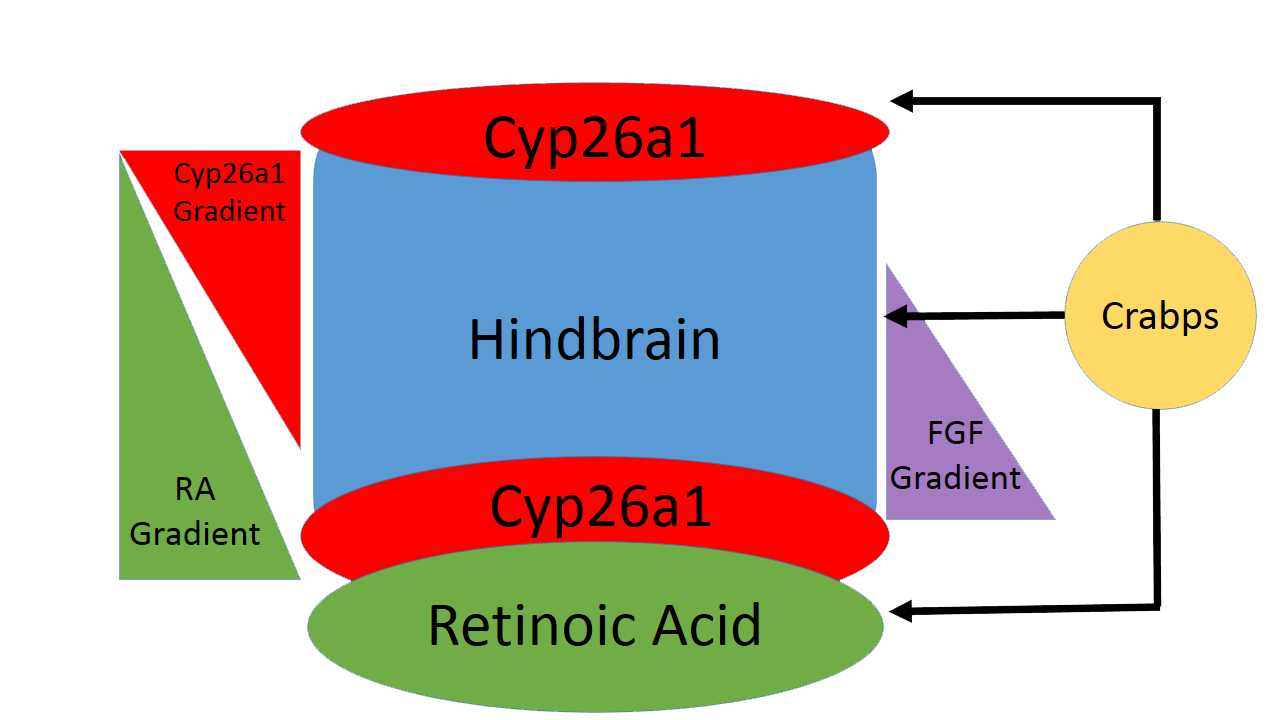
\includegraphics[scale=0.25]{figures/RAcartoons}
\par\end{center}